\documentclass[11pt,compress,t,notes=noshow, xcolor=table]{beamer}
\usepackage[]{graphicx}\usepackage[]{color}
% maxwidth is the original width if it is less than linewidth
% otherwise use linewidth (to make sure the graphics do not exceed the margin)
\makeatletter
\def\maxwidth{ %
  \ifdim\Gin@nat@width>\linewidth
    \linewidth
  \else
    \Gin@nat@width
  \fi
}
\makeatother

\definecolor{fgcolor}{rgb}{0.345, 0.345, 0.345}
\newcommand{\hlnum}[1]{\textcolor[rgb]{0.686,0.059,0.569}{#1}}%
\newcommand{\hlstr}[1]{\textcolor[rgb]{0.192,0.494,0.8}{#1}}%
\newcommand{\hlcom}[1]{\textcolor[rgb]{0.678,0.584,0.686}{\textit{#1}}}%
\newcommand{\hlopt}[1]{\textcolor[rgb]{0,0,0}{#1}}%
\newcommand{\hlstd}[1]{\textcolor[rgb]{0.345,0.345,0.345}{#1}}%
\newcommand{\hlkwa}[1]{\textcolor[rgb]{0.161,0.373,0.58}{\textbf{#1}}}%
\newcommand{\hlkwb}[1]{\textcolor[rgb]{0.69,0.353,0.396}{#1}}%
\newcommand{\hlkwc}[1]{\textcolor[rgb]{0.333,0.667,0.333}{#1}}%
\newcommand{\hlkwd}[1]{\textcolor[rgb]{0.737,0.353,0.396}{\textbf{#1}}}%
\let\hlipl\hlkwb

\usepackage{framed}
\makeatletter
\newenvironment{kframe}{%
 \def\at@end@of@kframe{}%
 \ifinner\ifhmode%
  \def\at@end@of@kframe{\end{minipage}}%
  \begin{minipage}{\columnwidth}%
 \fi\fi%
 \def\FrameCommand##1{\hskip\@totalleftmargin \hskip-\fboxsep
 \colorbox{shadecolor}{##1}\hskip-\fboxsep
     % There is no \\@totalrightmargin, so:
     \hskip-\linewidth \hskip-\@totalleftmargin \hskip\columnwidth}%
 \MakeFramed {\advance\hsize-\width
   \@totalleftmargin\z@ \linewidth\hsize
   \@setminipage}}%
 {\par\unskip\endMakeFramed%
 \at@end@of@kframe}
\makeatother

\definecolor{shadecolor}{rgb}{.97, .97, .97}
\definecolor{messagecolor}{rgb}{0, 0, 0}
\definecolor{warningcolor}{rgb}{1, 0, 1}
\definecolor{errorcolor}{rgb}{1, 0, 0}
\newenvironment{knitrout}{}{} % an empty environment to be redefined in TeX

\usepackage{alltt}
\newcommand{\SweaveOpts}[1]{}  % do not interfere with LaTeX
\newcommand{\SweaveInput}[1]{} % because they are not real TeX commands
\newcommand{\Sexpr}[1]{}       % will only be parsed by R



\usepackage[english]{babel}
\usepackage[utf8]{inputenc}

\usepackage{dsfont}
\usepackage{verbatim}
\usepackage{amsmath}
\usepackage{amsfonts}
\usepackage{bm}
\usepackage{csquotes}
\usepackage{multirow}
\usepackage{longtable}
\usepackage{booktabs}
\usepackage{enumerate}
\usepackage[absolute,overlay]{textpos}
\usepackage{psfrag}
\usepackage{algorithm}
\usepackage{algpseudocode}
\usepackage{eqnarray}
\usepackage{arydshln}
\usepackage{tabularx}
\usepackage{placeins}
\usepackage{tikz}
\usepackage{setspace}
\usepackage{colortbl}
\usepackage{mathtools}
\usepackage{wrapfig}
\usepackage{bm}
\usetikzlibrary{shapes,arrows,automata,positioning,calc,chains,trees, shadows}
\tikzset{
  %Define standard arrow tip
  >=stealth',
  %Define style for boxes
  punkt/.style={
    rectangle,
    rounded corners,
    draw=black, very thick,
    text width=6.5em,
    minimum height=2em,
    text centered},
  % Define arrow style
  pil/.style={
    ->,
    thick,
    shorten <=2pt,
    shorten >=2pt,}
}
\usepackage{subfig}


% Defines macros and environments
\usepackage{bbm}
% basic latex stuff
\newcommand{\pkg}[1]{{\fontseries{b}\selectfont #1}} %fontstyle for R packages
\newcommand{\lz}{\vspace{0.5cm}} %vertical space
\newcommand{\dlz}{\vspace{1cm}} %double vertical space
\newcommand{\oneliner}[1] % Oneliner for important statements
{\begin{block}{}\begin{center}\begin{Large}#1\end{Large}\end{center}\end{block}}


%new environments
\newenvironment{vbframe}  %frame with breaks and verbatim
{
 \begin{frame}[containsverbatim,allowframebreaks]
}
{
\end{frame}
}

\newenvironment{vframe}  %frame with verbatim without breaks (to avoid numbering one slided frames)
{
 \begin{frame}[containsverbatim]
}
{
\end{frame}
}

\newenvironment{blocki}[1]   % itemize block
{
 \begin{block}{#1}\begin{itemize}
}
{
\end{itemize}\end{block}
}

\newenvironment{fragileframe}[2]{  %fragile frame with framebreaks
\begin{frame}[allowframebreaks, fragile, environment = fragileframe]
\frametitle{#1}
#2}
{\end{frame}}


\newcommand{\myframe}[2]{  %short for frame with framebreaks
\begin{frame}[allowframebreaks]
\frametitle{#1}
#2
\end{frame}}

\newcommand{\remark}[1]{
  \textbf{Remark:} #1
}


\newenvironment{deleteframe}
{
\begingroup
\usebackgroundtemplate{
\includegraphics[width=\paperwidth,height=\paperheight]{../style/color/red.png}}
 \begin{frame}
}
{
\end{frame}
\endgroup
}
\newenvironment{simplifyframe}
{
\begingroup
\usebackgroundtemplate{
\includegraphics[width=\paperwidth,height=\paperheight]{../style/color/yellow.png}}
 \begin{frame}
}
{
\end{frame}
\endgroup
}\newenvironment{draftframe}
{
\begingroup
\usebackgroundtemplate{
\includegraphics[width=\paperwidth,height=\paperheight]{../style/color/green.jpg}}
 \begin{frame}
}
{
\end{frame}
\endgroup
}
% https://tex.stackexchange.com/a/261480: textcolor that works in mathmode
\makeatletter
\renewcommand*{\@textcolor}[3]{%
  \protect\leavevmode
  \begingroup
    \color#1{#2}#3%
  \endgroup
}
\makeatother

% \usepackage{bbm}
% basic latex stuff
\newcommand{\pkg}[1]{{\fontseries{b}\selectfont #1}} %fontstyle for R packages
\newcommand{\lz}{\vspace{0.5cm}} %vertical space
\newcommand{\dlz}{\vspace{1cm}} %double vertical space
\newcommand{\oneliner}[1] % Oneliner for important statements
{\begin{block}{}\begin{center}\begin{Large}#1\end{Large}\end{center}\end{block}}


%new environments
\newenvironment{vbframe}  %frame with breaks and verbatim
{
 \begin{frame}[containsverbatim,allowframebreaks]
}
{
\end{frame}
}

\newenvironment{vframe}  %frame with verbatim without breaks (to avoid numbering one slided frames)
{
 \begin{frame}[containsverbatim]
}
{
\end{frame}
}

\newenvironment{blocki}[1]   % itemize block
{
 \begin{block}{#1}\begin{itemize}
}
{
\end{itemize}\end{block}
}

\newenvironment{fragileframe}[2]{  %fragile frame with framebreaks
\begin{frame}[allowframebreaks, fragile, environment = fragileframe]
\frametitle{#1}
#2}
{\end{frame}}


\newcommand{\myframe}[2]{  %short for frame with framebreaks
\begin{frame}[allowframebreaks]
\frametitle{#1}
#2
\end{frame}}

\newcommand{\remark}[1]{
  \textbf{Remark:} #1
}


\newenvironment{deleteframe}
{
\begingroup
\usebackgroundtemplate{
\includegraphics[width=\paperwidth,height=\paperheight]{../style/color/red.png}}
 \begin{frame}
}
{
\end{frame}
\endgroup
}
\newenvironment{simplifyframe}
{
\begingroup
\usebackgroundtemplate{
\includegraphics[width=\paperwidth,height=\paperheight]{../style/color/yellow.png}}
 \begin{frame}
}
{
\end{frame}
\endgroup
}\newenvironment{draftframe}
{
\begingroup
\usebackgroundtemplate{
\includegraphics[width=\paperwidth,height=\paperheight]{../style/color/green.jpg}}
 \begin{frame}
}
{
\end{frame}
\endgroup
}
% https://tex.stackexchange.com/a/261480: textcolor that works in mathmode
\makeatletter
\renewcommand*{\@textcolor}[3]{%
  \protect\leavevmode
  \begingroup
    \color#1{#2}#3%
  \endgroup
}
\makeatother


%\usetheme{lmu-lecture}
\newcommand{\titlefigure}{figure/cart_intro_2.pdf}
\newcommand{\learninggoals}{
\item Know definition of a tree's node
\item Understand how split points are derived via empirical risk minimization
\item Know which losses can be applied for regression and classification
\item Know the connections between empirical risk minimization and impurity minimization}
\usepackage{../../style/lmu-lecture}

\let\code=\texttt
\let\proglang=\textsf

\setkeys{Gin}{width=0.9\textwidth}

\title{Introduction to Machine Learning}
% \author{Bernd Bischl, Christoph Molnar, Daniel Schalk, Fabian Scheipl}
\institute{\href{https://compstat-lmu.github.io/lecture_i2ml/}{compstat-lmu.github.io/lecture\_i2ml}}
\date{}

\setbeamertemplate{frametitle}{\expandafter\uppercase\expandafter\insertframetitle}



\begin{document}
% Set style/preamble.Rnw as parent.


% Load all R packages and set up knitr

% This file loads R packages, configures knitr options and sets preamble.Rnw as parent file
% IF YOU MODIFY THIS, PLZ ALSO MODIFY setup.Rmd ACCORDINGLY...








% Defines macros and environments
\input{../../latex-math/basic-math.tex}
\input{../../latex-math/basic-ml.tex}
\input{../../latex-math/ml-trees.tex}

%! includes: cart-intro

\lecturechapter{CART: Splitting Criteria}
\lecture{Introduction to Machine Learning}
\sloppy

\begin{frame}[fragile]{Trees}

\lz 

\begin{columns}
\begin{column}{0.5\textwidth}
Classification Tree:
\lz


\begin{knitrout}\scriptsize
\definecolor{shadecolor}{rgb}{0.969, 0.969, 0.969}\color{fgcolor}

{\centering 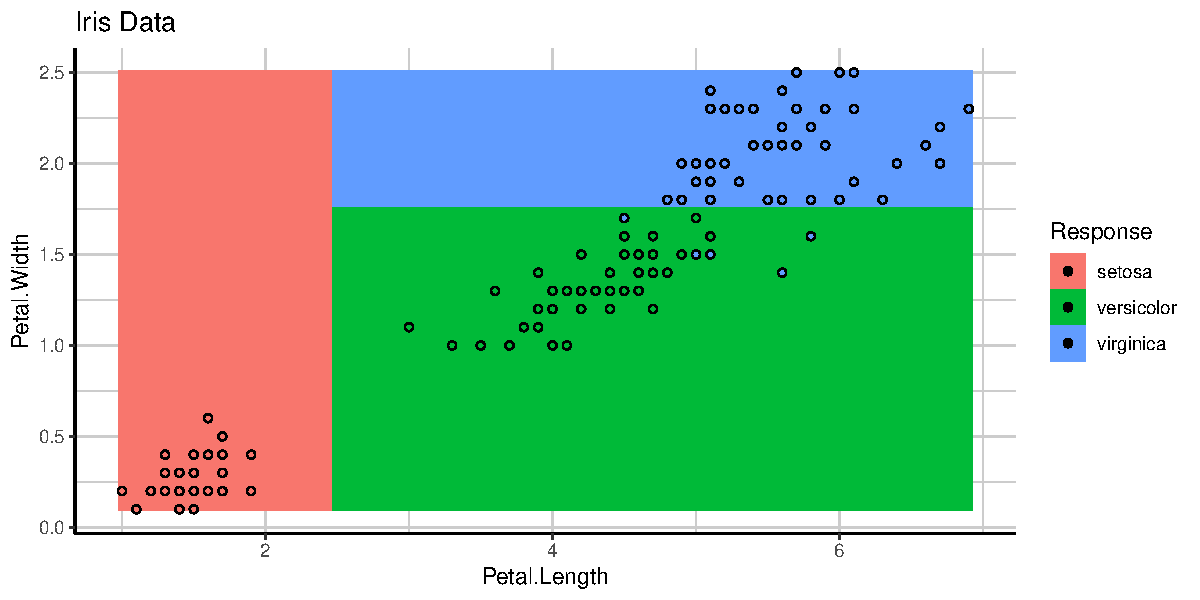
\includegraphics[width=0.95\textwidth]{figure/cart_splitcriteria_1} 

}



\end{knitrout}
 
\end{column}
\begin{column}{0.5\textwidth}
Regression Tree:

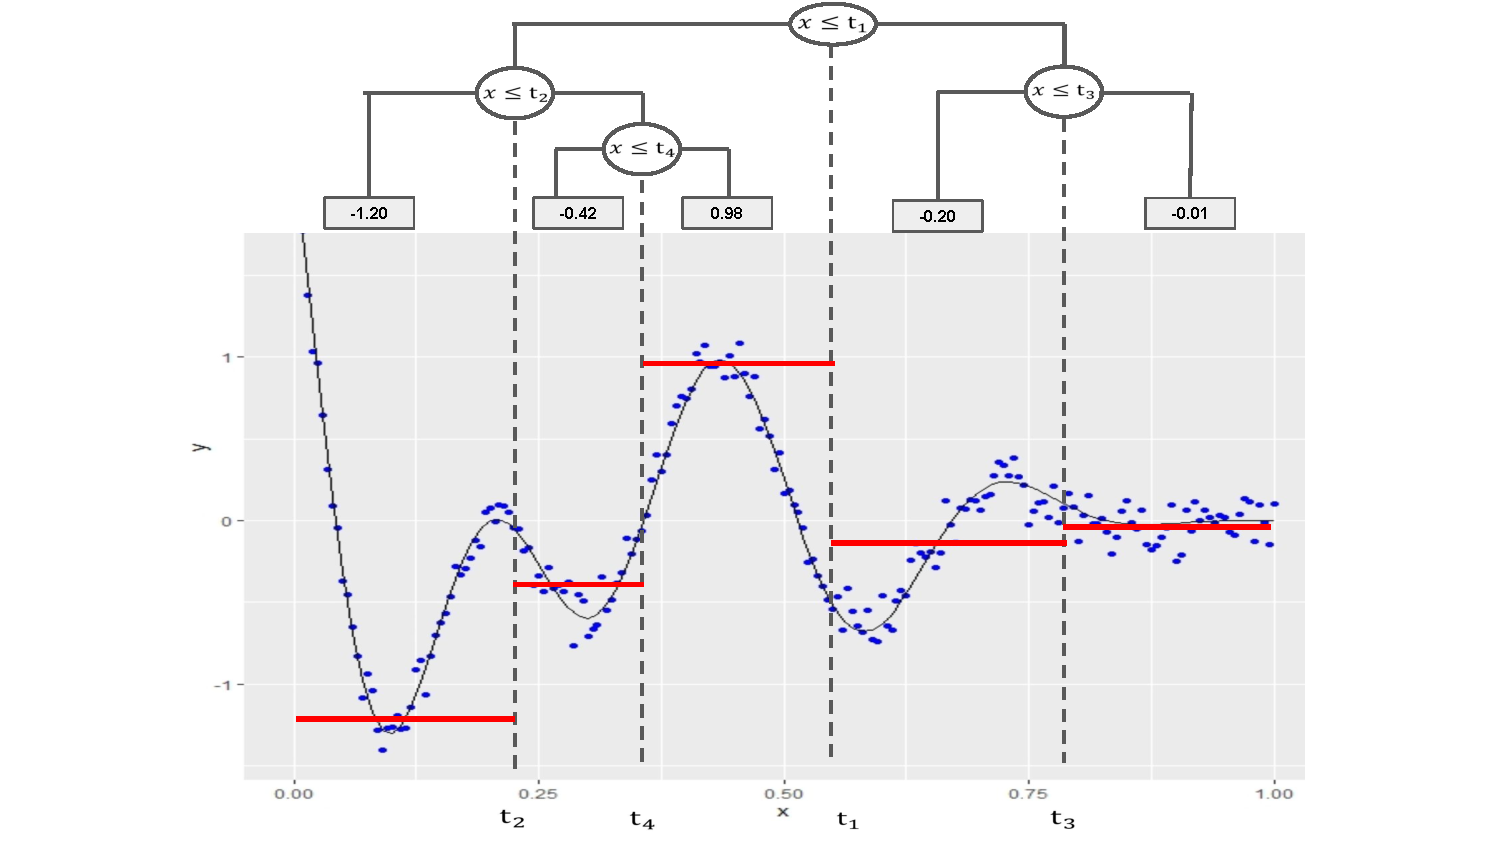
\includegraphics[height = 0.4\textheight]{figure_man/CART_reg_example.pdf}

\end{column}
\end{columns}
\end{frame}

\begin{frame}{Splitting criteria}

 \begin{figure}
    \centering
      % FIGURE SOURCE: No source
      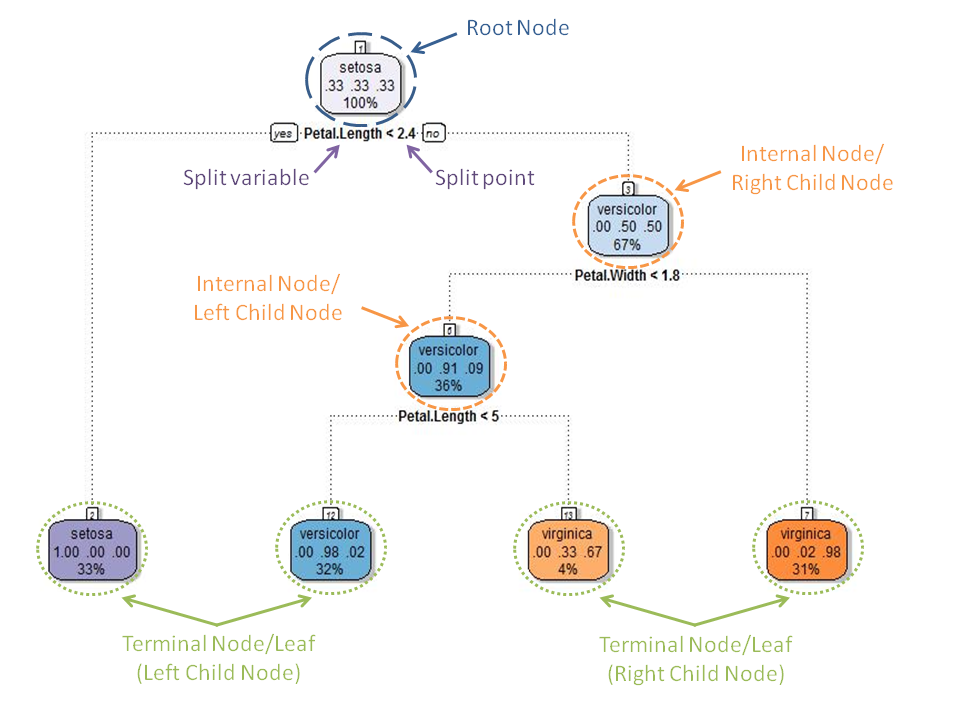
\includegraphics[height = 5.0cm]{figure_man/labelling_of_tree.png}
    \end{figure}

How to find good splitting rules to define the tree?
\lz

$\implies$ \textbf{empirical risk minimization}

\end{frame}

\begin{vbframe}{Splitting criteria: Formalization}

\begin{itemize}
\item Let $\Np \subseteq \D$ be the data that is assigned to a terminal node $\Np$ of a tree.
\item Let $c$ be the predicted constant value for the data assigned to $\Np$: $\yh \equiv c$ for all $\left(\xv, y\right) \in \Np$.
\item Then the risk $\risk(\Np)$ for a leaf is simply the average loss for the data assigned to that leaf under a given loss function $L$:
  $$\risk(\Np) = \frac{1}{|\Np|} \sum\limits_{(\xv, y) \in \Np} L(y, c)$$
\item The prediction is given by the optimal constant $c = \argmin_c \risk(\Np)$
\end{itemize}

\framebreak

\begin{itemize}
\item A split w.r.t. \textbf{feature $x_j$ at split point $t$} divides a parent node $\Np$ into 
  \begin{align*}
    \Nl &= \{ (\xv, y) \in \Np: x_j \leq t \} \text{ and } \Nr = \{ (\xv, y) \in \Np: x_j > t \}.
  \end{align*}
\item   
  In order to evaluate how good a split is, we compute the empirical risks
  in both child nodes and sum them up:
     \begin{align*}
      \risk(\Np, j, t) &= \frac{|\Nl|}{|\Np|} \risk(\Nl) + \frac{|\Nr|}{|\Np|} \risk(\Nr) \\
                  &= \frac{1}{|\Np|}\left(\sum\limits_{(\xv,y) \in \Nl} L(y, c_1) + \sum\limits_{(\xv,y) \in \Nr} L(y, c_2)\right)
      \end{align*}
  \item Finding the best way to split $\Np$ into $\Nl, \Nr$ means solving
  $$\argmin_{j, t} \risk(\Np, j, t)$$
\end{itemize}
\end{vbframe}

\begin{vbframe}{Splitting criteria: Regression}
\begin{itemize}
 \item For regression trees, we usually use $L_2$ loss:
  $$\risk(\Np) = \frac{1}{|\Np|} \sum\limits_{(\xv,y) \in \Np} (y - c)^2$$
 \item The best constant prediction under $L_2$ is the mean:
  $$c = \bar{y}_\Np = \frac{1}{|\Np|} \sum\limits_{(\xv,y) \in \Np} y$$
\end{itemize}

\framebreak

\begin{itemize}
\item This means the best split is the one that minimizes the (pooled) variance of the target distribution in the child nodes $\Nl$ and $\Nr$:
\begin{knitrout}\scriptsize
\definecolor{shadecolor}{rgb}{0.969, 0.969, 0.969}\color{fgcolor}

{\centering 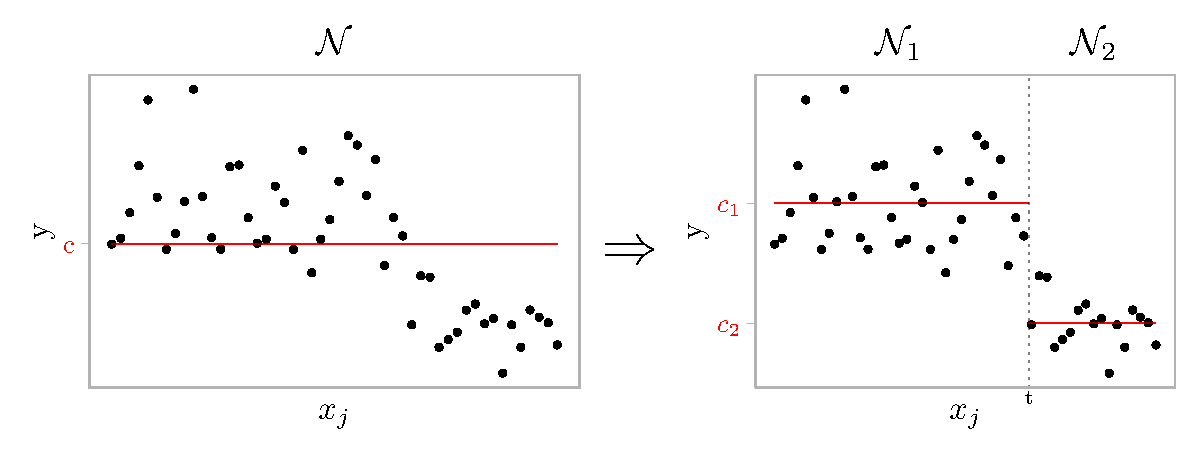
\includegraphics[width=0.95\textwidth]{figure/cart_splitcriteria_2.pdf} 

}



\end{knitrout}
We can also interpret this as a way of measuring the impurity of the target distribution, i.e., how much it diverges from a constant in each of the child nodes.
\item For $L_1$ loss, $c$ is the median of $y \in \Np$.
\end{itemize}
\end{vbframe}

\begin{vbframe}{Splitting Criteria: Classification}

\begin{itemize}
\item Typically uses either Brier score (so: $L_2$ loss on probabilities) or  Bernoulli loss (as in logistic regression) as loss functions
\item Predicted probabilities in node $\Np$ are simply the class proportions in the node:
$$ \pikNh = \frac{1}{|\Np|} \sum\limits_{(\xv,y) \in \Np} \I(y = k) $$
This is the optimal prediction under both the logistic / Bernoulli loss and the Brier loss.
\end{itemize}

\begin{knitrout}\scriptsize
\definecolor{shadecolor}{rgb}{0.969, 0.969, 0.969}\color{fgcolor}

{\centering 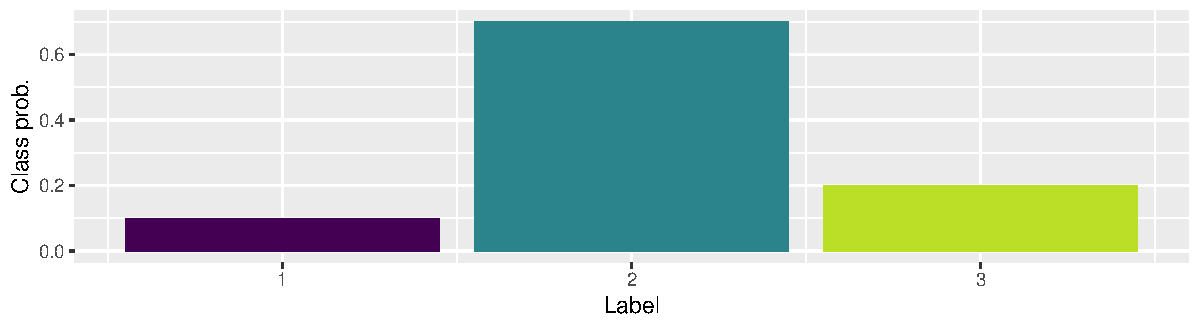
\includegraphics[width=0.95\textwidth]{figure/cart_splitcriteria_3} 

}



\end{knitrout}
\end{vbframe}

\begin{vbframe}{Splitting Criteria: Comments}

\begin{itemize}
\item Splitting criteria for trees are usually defined in terms of "impurity reduction". Instead of minimizing empirical risk in the child nodes over all possible splits, a measure of \enquote{impurity} of the distribution of the target $y$ in the child nodes is minimized. 
\item For regression trees, the \enquote{impurity} of a node is usually defined as the variance of the $\yi$ in the node. Minimizing this \enquote{variance impurity} is equivalent to minimizing the squared error loss for a predicted constant in the nodes. 

\framebreak 

\item Minimizing the Brier score is equivalent to minimizing the Gini impurity
$$I(\Np) = \sumkg \pikNh \left( 1-\pikNh \right)$$
\item Minimizing the Bernoulli loss is equivalent to minimizing entropy impurity
$$I(\Np) = -\sumkg \pikNh \log \pikNh$$
\item The approach based on loss functions instead of impurity measures is simpler and more straightforward, mathematically equivalent and shows that growing a tree can be understood in terms of empirical risk minimization.
\end{itemize}
\end{vbframe}

\begin{vbframe}{Splitting with misclassification loss}

\begin{itemize}
\item Why don't we use the misclassification loss for classification trees? I.e., always predict the majority class in each child node and count how many errors we make.
\item In many other cases, we are interested in minimizing this kind of error but have to approximate it by some other criterion instead, since the misclassification loss does not have derivatives that we can use for optimization.\\
We don't need derivatives when we optimize the tree, so we could go for it!
\item This is possible, but Brier score and Bernoulli loss are more sensitive to changes in the node probabilities, and  therefore often preferred
\end{itemize}

\framebreak

Example: two-class problem with 400 obs in each class and two possible splits:
\begin{small}
\begin{columns}[T,onlytextwidth]
\column{0.5\textwidth}
\begin{center}
\textbf{Split 1:} \\
\vspace{0.25cm}
% latex table generated in R 4.0.1 by xtable 1.8-4 package
% Mon Aug 10 01:13:29 2020
\begin{table}[ht]
\centering
\begin{tabular}{rrr}
  \hline
 & class 0 & class 1 \\ 
  \hline
$\Nl$ & 300 & 100 \\ 
  $\Nr$ & 100 & 300 \\ 
   \hline
\end{tabular}
\end{table}

\end{center}
\column{0.5\textwidth}
\begin{center}
\textbf{Split 2:} \\
\vspace{0.25cm}
% latex table generated in R 4.0.1 by xtable 1.8-4 package
% Mon Aug 10 01:13:29 2020
\begin{table}[ht]
\centering
\begin{tabular}{rrr}
  \hline
 & class 0 & class 1 \\ 
  \hline
$\Nl$ & 400 & 200 \\ 
  $\Nr$ &   0 & 200 \\ 
   \hline
\end{tabular}
\end{table}

\end{center}
\end{columns}
\end{small}

\lz

\begin{itemize}
\item Both splits are equivalent in terms of misclassification error, they each misclassify 200 observations. 
\item But: Split 2 produces one pure node and is probably preferable.
\item Brier loss (Gini impurity) and Bernoulli loss (entropy impurity) prefer the second split
\item Calculation for Gini:\\
\begin{alignat*}{6}
\text{Formula}&:& \frac{|\Nl|}{|\Np|}\cdot 2 \cdot\pikNlh[0]\pikNlh[1] &+& \frac{|\Nr|}{|\Np|}\cdot 2 \cdot \pikNrh[0]\pikNrh[1] &=& \\[5ex]
\text{Split 1}&:& \,\, \frac{1}{2} \,\cdot \, 2 \,\cdot\, \frac{3}{4} \,\cdot\, \frac{1}{4} \,&+&\,  \, \frac{1}{2} \,\cdot\, 2 \, \cdot\, \frac{1}{4} \,\cdot\, \frac{3}{4} &=&\;\, \frac{3}{8}\\[5ex]
\text{Split 2}&:& \frac{3}{4}\, \cdot\, 2 \,\cdot\,\frac{2}{3}\,\cdot\,\frac{1}{3}\, &+& \frac{1}{4} \,\cdot\, 2 \,\cdot\, 0 \,\cdot\, 1 &=&\; \,\frac{1}{3}
% (Brier not introduced)
%$Split1: 300(0-\frac{1}{4})^2 + 100(1-\frac{1}{4})^2 + 100(0-\frac{3}{4})^2+300(1-\frac{3}{4})^2 = 150$\\ 
%$Split2: 400(0-\frac{1}{3})^2 + 200(1-\frac{1}{3})^2 = 133.3$
\end{alignat*}
\end{itemize}
\end{vbframe}

 
 




\endlecture
\end{document}
